\documentclass[a4paper,12pt]{article}
\usepackage[utf8]{inputenc}
\usepackage[T2A]{fontenc}
\usepackage[russian]{babel}
\usepackage{geometry}
\geometry{left=2cm,right=2cm,top=2cm,bottom=2cm}
\usepackage{titlesec}
\usepackage{enumitem}
\usepackage{parskip}
\usepackage{graphicx} % Для изображений
\usepackage{wrapfig} % Для размещения фото

\titleformat{\section}{\large\bfseries}{\thesection}{1em}{}
\setlength{\parindent}{0pt}
\setlist[itemize]{leftmargin=*}
\setlist[enumerate]{leftmargin=*}

\usepackage{times}

\begin{document}

% Header with photo
\begin{center}
    \begin{wrapfigure}{r}{3cm}
        \vspace{-20pt}
        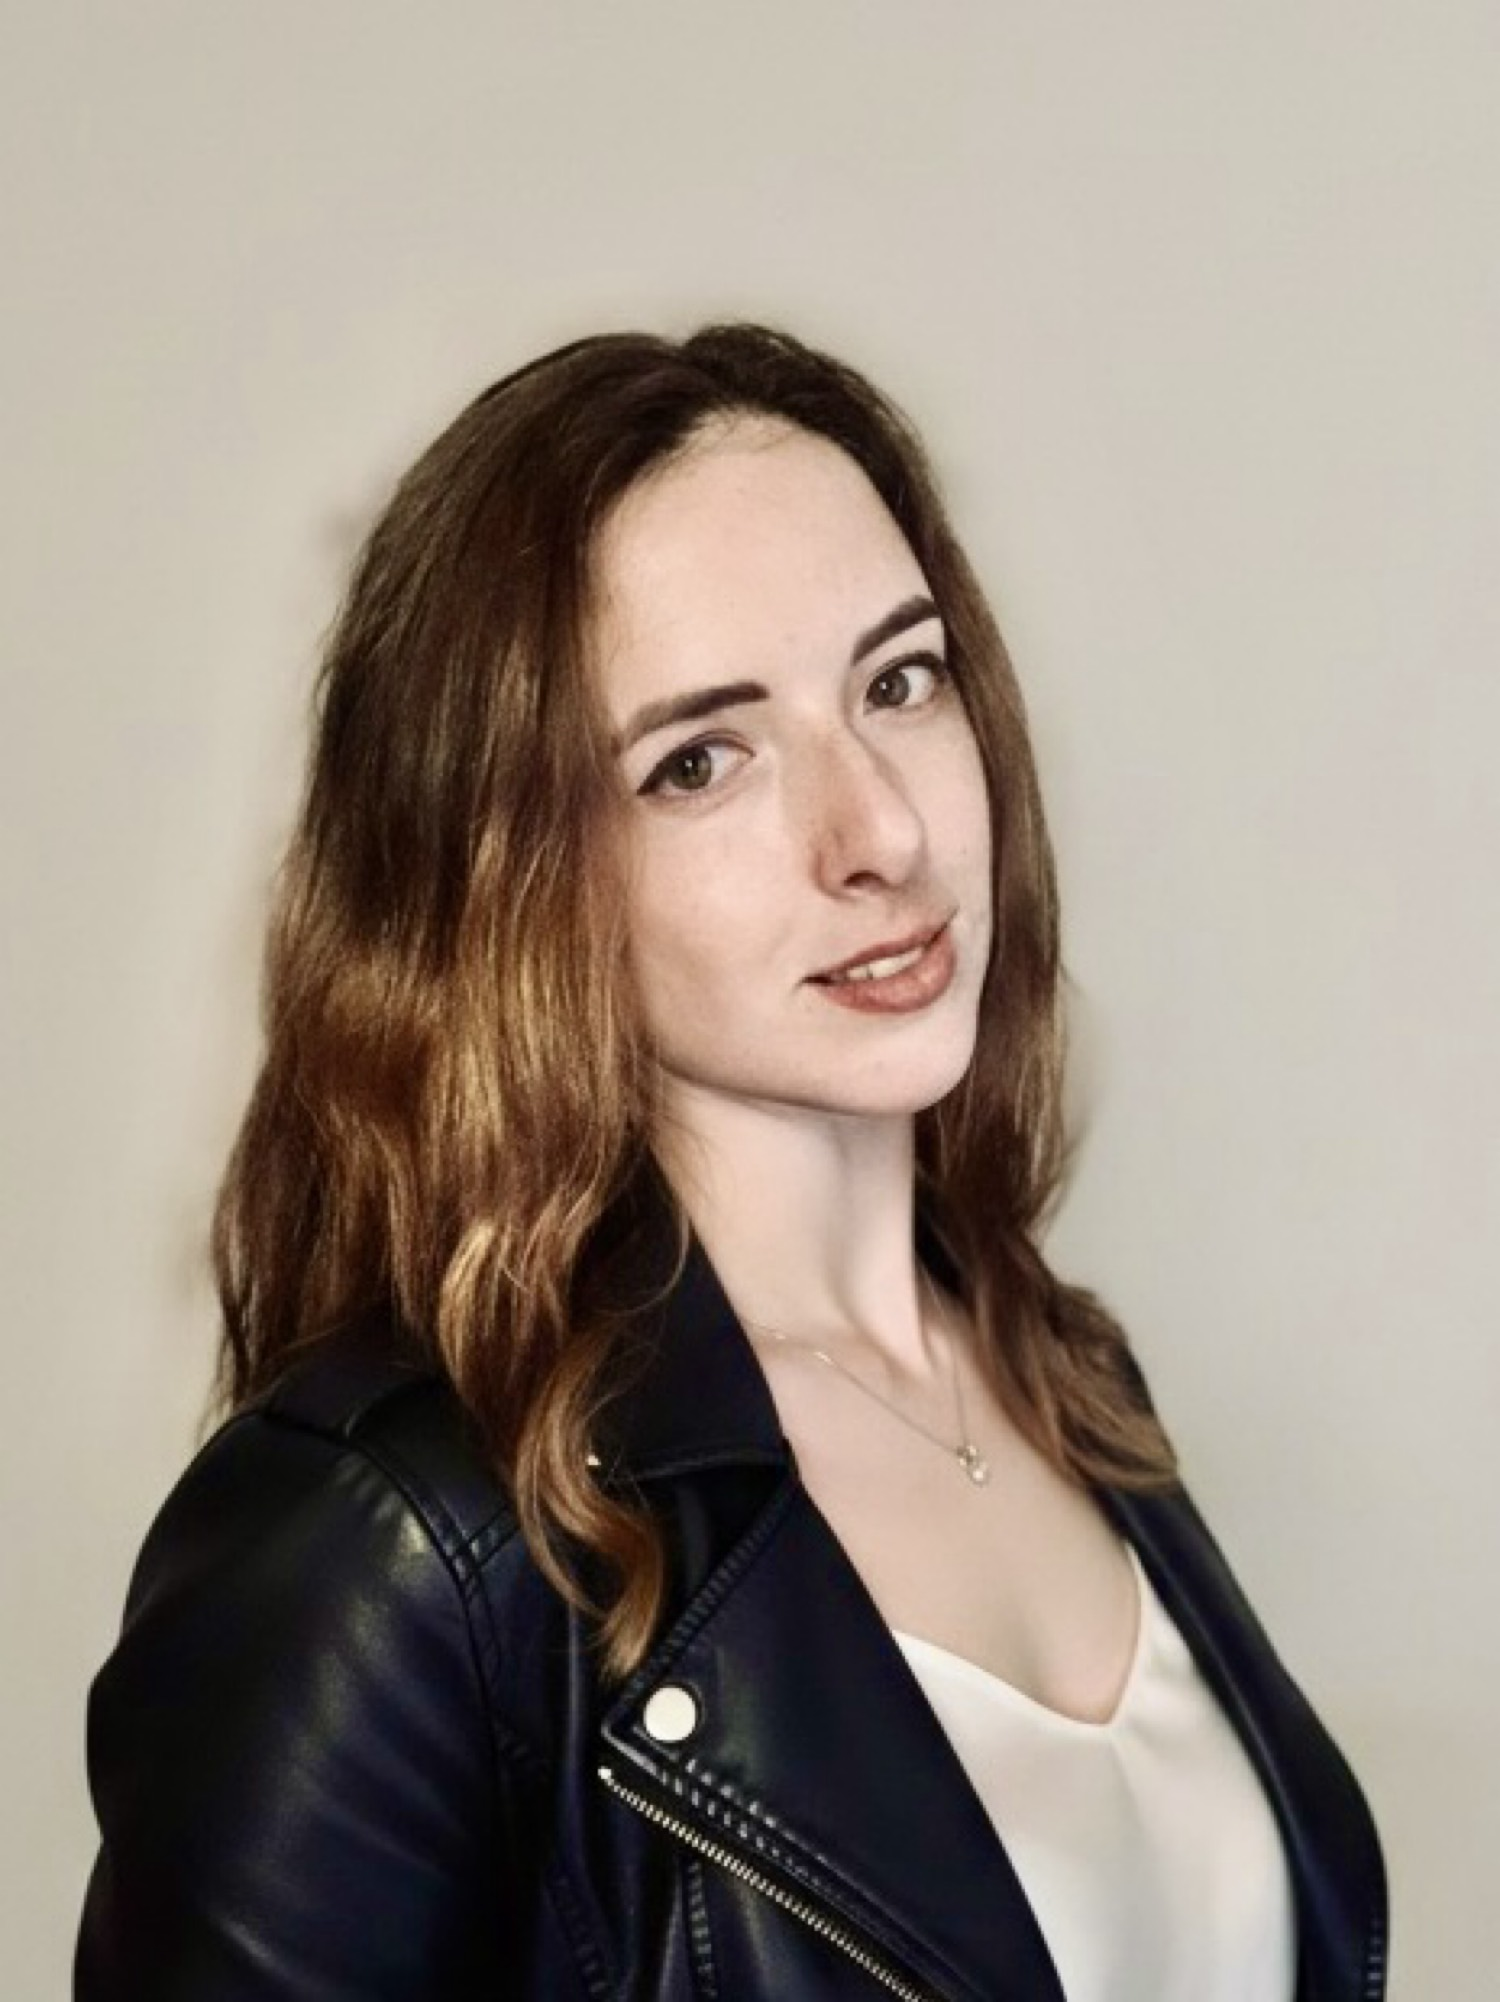
\includegraphics[width=3cm]{my-photo.jpg}
    \end{wrapfigure}
    {\LARGE\bfseries Киселёва Мария Васильевна} \\[0.2cm]
    Брест, Беларусь | +375291155818 | m.yasinskaya12@gmail.ru | 12 мая 1994
\end{center}

\section{Цель}
Ищу позицию в сфере IT, с фокусом на промт-инженерию, веб-разработку или аналитику. Стремлюсь применять навыки HTML, CSS и Python, развиваться в создании нейросетевых решений и вносить вклад в инновационные проекты. Готова к самостоятельному ведению несложных проектов или работать в команде разработчиков.

\section{Навыки и качества}
\begin{itemize}
    \item Быстрая обучаемость и адаптация к новым технологиям
    \item Уверенное владение HTML и CSS
    \item Базовые навыки программирования на Python
    \item Опыт в маркетинге и продажах
    \item Аналитическое мышление и внимание к деталям
    \item Коммуникабельность и умение работать в команде
    \item Организованность и управление временем
    \item Креативность в решении задач
\end{itemize}

\section{Образование и курсы}
\begin{itemize}
    \item \textbf{Курс «Введение в нейросети»}, онлайн-платформа, 2024
    \item \textbf{Курс «Нейросети в бизнесе»}, онлайн-платформа, в процессе, 2025
    \item \textbf{Курс по маркетингу}, туристическое агентство, 2022
    \item \textbf{Курс по технике продаж}, компания по продаже часов и ювелирных украшений, 2020
\end{itemize}

\section{Опыт работы}
\begin{itemize}
    \item \textbf{Менеджер по туризму и маркетингу}, Туристическое агентство, Брест, 2021--2023
    \begin{itemize}
        \item Разрабатывала маркетинговые кампании, увеличившие поток клиентов на 15\%
        \item Вела переговоры с партнёрами и клиентами
        \item Прошла курс по маркетингу для оптимизации стратегий
    \end{itemize}
    \item \textbf{Продавец-консультант}, Компания по продаже часов и ювелирных украшений, Брест, 2019--2021
    \begin{itemize}
        \item Консультировала клиентов, увеличивая продажи на 20\% за счёт техник продаж
        \item Прошла курс по технике продаж, применила знания для повышения клиентской лояльности
    \end{itemize}
    \item \textbf{Администратор}, Салон красоты, Брест, 2017--2019
    \begin{itemize}
        \item Организовывала работу персонала и вела клиентскую базу
        \item Оптимизировала расписание, сократив время ожидания клиентов на 30\%
    \end{itemize}
\end{itemize}

\section{Дополнительно}
\begin{itemize}
    \item Уровень английского языка: B2 (Upper-Intermediate)
    \item Водительские права: категории A, B
    \item Активно изучаю Python, готова участвовать в разработке в составе команды
    \item Увлечена промт-инженерией, стремлюсь применять нейросети в бизнесе
    \item Свободно работаю с HTML и CSS, создаю адаптивные веб-страницы
    \item Готова к обучению новым технологиям и вызовам
\end{itemize}

\end{document}